\part{SİMÜLASYON MODELİ}
\thispagestyle{empty}
\newpage
\section{YENİLENEBİLİR ENERJİ SİSTEMLERİNDE KULLANILAN ALGILAYICILARIN VERİ YAPILARI}

Yenilenebilir enerji sistemlerinde veri transfer standartlarını oluşturabilmek için \gls{iec} 61850 iletişim standardı kullanılır. İlgili standart kullanılarak enerji santrallerinde oluşturulan veriler kontrol, gözlem ve enerji sistemlerinde oluşabilecek arızaların gerçek zamanlı şekilde kontrolünün sağlanması amaçlanmıştır \cite{1385190}. Rüzgar enerji türbinleri ve güneş enerji panellerinde oluşturulacak sistemsel çalışma verilerinin aktif bir şekilde kontrolü amaçlanmıştır. Bu kontrolün sağlanması için \gls{iec} 61850 ve benzer standartlardan olan \gls{iec} 61400-25 standartları dikkate alınmıştır \cite{Olsen_prototypeof} \cite{francisco2016protection}.


\subsection{Rüzgar Enerji Sistemlerinde Veri Yapıları}
Eskiden, rüzgar enerji türbinleri ile kontrol odası arasındaki iletişim sistemi, enerji üretimi işini yüklenen firmalar tarafından belirli bir standarda bağlı olmadan çözül-mekteydi. Bu durum yüklenici firmaların hepsinde kendisine özel bir çözüm oluşturmaya sebebiyet vermiştir. Danimarkalı büyük bir türbin firması ilgili haberleşme çözümü için \gls{iec}'ye başvuruda bulunmuştur. Bu başvuru sayesinde \gls{res}'lerin haberleşme standarlarından \gls{iec} 61400 standardı geliştirilmiştir \cite{Olsen_prototypeof}.

\gls{iec} 61400-25 standardı, rüzgar enerjisi santrallerinin izlenmesi ve kontrolü için birleşik bir iletişim sisteminin tanımlanması ve standartlaştırılması için özel bir versiyondur. \gls{iec} 61400-25 serisi, genel olarak trafo merkezlerindeki iletişim ağlarını ve sistemleri tanımla-yan \gls{iec} 61850 serisi standartların bir uzantısıdır. 


\gls{iec} 61400-25 standardı sayesinde, enerji üretim sistemindeki algılayıcılardan oluşan veriler sayısal haberleşme standartlarında tekrardan yapılandırılıp komuta kontrol merkezlerine iletilir. IEC 61400 5 kategoriye ayrılır.

•	Genel tanımlar ilkeler ve modeller (\gls{iec} 61400-25-1).

•	Rüzgar türbinlerinin enformasyon model standardı (\gls{iec} 61400-25-2).

•	Enformasyon değişim model standardı (\gls{iec} 61400-25-3).

•	İletişim profilinde uyumluluk standardı (\gls{iec} 61400-25-4).

•	Rüzgar enerji santrallerinde izleme ve kontrol altyapısının uygunluk testleri (\gls{iec} 61400-25-5).

%\gls{res}'teki kontrol ve durum raporu için çalışan mantıksal düğümlerin veri sınıflandırılması \cite{Olsen_prototypeof}.

\subsection{\gls{iec} 61400-25-2 Standardı}

Enformasyon modeli standardı sayesinde rüzgar enerji santrallerinin faaliyeti sırasında yapılan ölçüm ve durum değerleri veri iletişimine hazır hale getirilir. Buna göre enerji santralinde kullanılan tüm donanımlara ait bir veri yapısı oluşturulur. \gls{iec} 61850 standardına göre belirtilen veri haberleşme standardıyla birlikte 61400-25 standardı birlikte incelendiğinde, bir rüzgar enerji türbininde üretilen veriler dokuz adet farklı modülde toplanmaktadır. İlgili modüllerin kısaltması Şekil \ref{fig:figure15}’de gösterilmiştir. Tablo \ref{tab:tabb2}’de türbin içi modüllerin açıklaması ve algılayıcı sayıları gösterilmiştir \cite{francisco2016protection}\cite{trinnass}\cite{san2007use}.



\begin{figure}[htbp]
\centerline{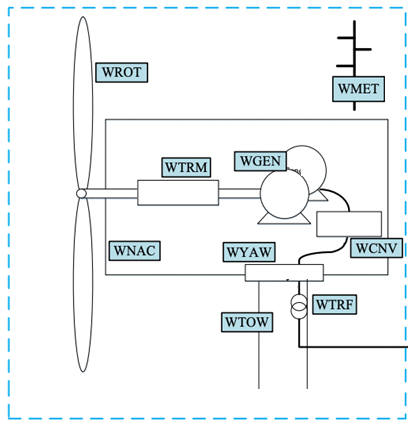
\includegraphics[width=7cm]{Resim/Sekil4-1.png}}
\caption{IEC 61400 standardına göre Türbin içerisindeki  algılayıcı düğümlerin gösterimi (\protect\citeA{jannasch2009daten}).}
\label{fig:figure15}
\end{figure}

\gls{iec} 61850 ve \gls{iec} 61400 standartları dikkate alındığında bir rüzgar türbininin sağlıklı bir şekilde çalışması için üzerinde faal durumda olması gereken 79 analog, 32 adet durum algılayıcısı bulunmalıdır. Tablo \ref{tab:tabb2}’de bir rüzgar türbininde bulunan algılayıcıların sayıları ve bağlı oldukları modüller gösterilmiştir. Tablo \ref{tab:WNACdetay}’de türbin içi modüllerden \gls{wnac}, rüzgar türbinlerinin pal kısmını kapsayan motor mekanizmasına ait modüldür. Bu modüle ait 4 durum ve 11 adet analog algılayıcı bulunmaktadır. WNAC modülüne ait algılayıcıların yerleşim detayı Şekil \ref{fig:4-2}'de, algılayıcıların tanımı ise Tablo \ref{tab:WNACdetay}’de gösterilmiştir. 
\cite{francisco2016protection}\cite{trinnass}\cite{san2007use}.


\begin{table}[htbp]
\centering
\caption{Türbin içi mantıksal düğüm özellikleri}
\label{tab:tabb2}
\begin{tabular}{ccccc}
\begin{tabular}[c]{@{}c@{}}Modül\\ İsmi\end{tabular} &
  \begin{tabular}[c]{@{}c@{}}Modül\\ Tanımı\end{tabular} &
  \begin{tabular}[c]{@{}c@{}}Zorunlu/\\ Opsiyonel\end{tabular} &
  \begin{tabular}[c]{@{}c@{}}Durum\\ Algılayıcı\\ Sayısı\end{tabular} &
  \begin{tabular}[c]{@{}c@{}}Analog\\ Algılayıcı\\ Sayısı\end{tabular} \\ \hline
WROT & Türbin rotor modülü       & Zorunlu   & 5 & 12 \\
WTRM & Türbin şanzıman modülü    & Opsiyonel & 8 & 12 \\
WGEN & Türbin jeneratör modülü   & Zorunlu   & 2 & 14 \\
WCNV & Türbin dönüştürücü modülü & Opsiyonel & 2 & 15 \\
WTRF & Türbin trafo modülü       & Opsiyonel & 3 & 8  \\
\gls{wnac} & Türbin motor modülü       & Zorunlu   & 4 & 11 \\
WYAW & Türbin yön ve açı modülü  & Zorunlu   & 2 & 6  \\
WTOW & Türbin kule modülü        & Opsiyonel & 3 & 2  \\
WMET & Türbin meteoroloji modülü & Zorunlu   & 0 & 8 
\end{tabular}
\end{table}


\begin{table}[htbp]
\centering
\caption{\gls{wnac} modülüne ait algılayıcıların tanımı \gls{iec} 61400-25 std.}
\label{tab:WNACdetay}
\begin{tabular}{ll}
\multicolumn{2}{l}{Durum algılayıcıları}        \\ \hline
BecBulbSt & İndikatör                           \\
WdHtSt    & Rüzgar algılayıcı ısıtıcı durumu    \\
IceSt     & Buz algılayıcı durumu               \\
AveSt     & Birinci ve ikinci anemometre durumu \\
\multicolumn{2}{l}{Analog algılayıcıları}           \\ \hline
Dir       & Türbin pal yönü                     \\
WdSpd     & Motor dışı rüzgar hızı              \\
WdDir     & Motor dışı rüzgar yönü              \\
ExTmp     & Modor dış sıcaklığı                 \\
IntlTmp   & Motor iç sıcaklığı                  \\
IntlHum   & Motor iç nemi                       \\
BecLumLev & Uyarı ışığı lüks değeri             \\
Vis       & Motor dışı görüş netlik değeri      \\
Ice       & Buz kalınlığı                       \\
DispXdis  & Kule yön değişikliği yatay açı      \\
DispYdir  & Kule yön değişikliği dikey açı      \\ \hline
\end{tabular}
\end{table}


\subsection{Güneş Enerji Sistemlerinde Veri Yapıları}
Güneş enerji sistemlerinde üretilen enerjinin takibi ve kontrolü için \gls{iec} 61724 standardı oluşturulmuştur. İlgili standardın amacı;

•	Fotovoltaik sistemdeki performans trendlerinin belirlenmesi.

•	Fotovoltaik sistemdeki olası arızaların lokalizasyonu.

•	Fotovoltaik sistem performansının tasarım beklentileri ve garantileriyle karşı-laştırılması.

•	Farklı konfigürasyonlardaki fotovoltaik sistemlerin karşılaştırılması.

•	Farklı lokasyonlardaki fotovoltaik sistemlerin karşılaştırılması 
olarak tanımla-nabilir. \cite{klise2017application} \cite{iec_2019} 

Bahsedilen amaçlar doğrultusunda tasarlanan güneş enerji sistemlerinde, performans analizlerinin yapılması hataların kolayca tespit edilmesi ve benzeri bir çok görevin başarıyla tamamlanmasına imkan vermektedir. \gls{iec} 61724 standardına göre izleme sistemi, güneş enerjisi sisteminin boyutuna ve kullanıcı gereksinimlerine göre uyarlanması gerektiğini belirtir \cite{trinnass}.

Genel olarak, daha büyük ve daha pahalı \gls{ges}, daha küçük ve daha düşük mali-yetli güneş enerjisi sistemlerinden daha fazla izleme noktasına ve daha yüksek doğrulukta algılayıcılara sahip olmalıdır. Bu gereksinime göre güneş enerji sistemleri A sınıfı, B sınıfı ve C sınıfı olarak üç sınıfta incelenir. Güneş enerji sistemlerinde çalışan algılayı-cıların genel olarak örnekleme ve veri gönderme periyotlarının maksimum değerleri Tablo \ref{tab:tablo4-3}’de gösterilmiştir.


\begin{table}[htbp]
\centering
\caption{Güneş tarlasında kullanılan algılayıcıların özellikleri}
\label{tab:tablo4-3}
\begin{tabular}{lccc}
Algılayıcı sınıfları &
  \multicolumn{1}{l}{\begin{tabular}[c]{@{}l@{}}A sınıfı (Yüksek\\ tutarlılık periyodu)\end{tabular}} &
  \multicolumn{1}{l}{\begin{tabular}[c]{@{}l@{}}B sınıfı (Orta\\ tutarlılık periyodu)\end{tabular}} &
  \multicolumn{1}{l}{\begin{tabular}[c]{@{}l@{}}C sınıfı (Düşük\\ tutarlılık periyodu)\end{tabular}} \\ \hline
Radyant ışıma        & 3s  & 60s & 60s \\
Meteorolojik         & 3s  & 60s & 60s \\
Rüzgar değerleri     & 3s  & 60s & 60s \\
Elektriksel değerler & 3s  & 60s & 60s \\
Kirlenme değerleri   & 60s & 60s & 60s
\end{tabular}
\end{table}


Tablo \ref{tab:tablo4-3}’de gösterilen algılayıcı sınıflarından yola çıkılarak 2015 senesinde yazılan bir makalede küçük çaplı güneş enerji sistemlerinde kullanılan algılayıcıların haber-leşme analizi yapılmıştır. \cite{ahmed2015communication}

\section{OPNET Yazılımı}

Günümüzde \gls{iot} ve veri haberleşmesinin boyutlarının her geçen gün artması nedeniyle şirketlerin haberleşme sistemlerine yapmış olduğu yatırımların büyüklüğü artmakta olduğu bilinmektedir. Haberleşme çözümleri için kullanılan donanımların sayısı arttıkça kurulum maliyeti ve sistemsel bir aksamanın oluşturacağı maliyet orantılı bir şekilde artacaktır. Buna göre araştırmacılar bir haberleşme sisteminin sahada kurulum aşamasından önce simülasyon ortamında tasarlanarak ilgili maliyetlerin fizibilitesini yapabilecekleri yazılımlar tasarlamışlardır. \gls{opnet} şimdiye kadar tasarlanmış en popüler ağ simülatör yazılımıdır. \gls{opnet} ticari bir yazılımdır ve ticari amaçlarla kullanılmasından kaynaklı olarak, OPNET hakkında yazılmış çok fazla makale ve kitap bulunmaktadır \cite{lu2012unlocking}\cite{sethi2012practical}. 

\begin{comment}
\subsection{OPNET Yazılımının Özellikleri}

•	Kolay bir grafik arayüzüne sahiptir.

•	Kullanıcılara zengin bir ağ modeli ve ağ tasarım kütüphanesi sunmaktadır.

•	Kullanıcı kolayca senaryo analizi yapabilmektedir.

•	Kurulumu diğer ağ tasarım programlarına göre daha kolaydır.

•	Grafik arayüzleri sayesinde sanal gerçek zamanlı ortam sağlar.

•	Ticari bir program olmasından kaynaklı, güvenilir ve verimlidir.

\end{comment}




\subsection{OPNET Yazılımında Algılayıcı Düğümlerin Modellenmesi}

Rüzgar türbinlerinde ve güneş enerjisi tarlalarında gözlem ve durum analizinin kolayca uygulanması için bir takım algılayıcı modüller \gls{iec} 61400, \gls{iec} 61724 ve \gls{iec} 61850 standartlarına göre oluşturulmuştur\cite{ahmed2011simulation}. \gls{iec} 61400 standardı dikkate alınarak bir rüzgar enerji türbininin OPNET yazılımında simülasyonu yapılmıştır. Bu çalışmada tasarlanan algılayıcı düğümlerinin Ethernet standartlarına göre haberleşme altyapısı oluşturulmuş 10BaseT, 100BaseT ve 1000BaseX standartlarındaki haberleşme hızlarına göre performansı incelenmiştir.
Kütahya Dumlupınar Üniversitesi'ndeki uzak yerleşkelere kurulacak güneş ve rüzgar enerji sistemlerindeki algılayıcıların tasarımında ilgili makalede bahsedilen teknikler kullanılmıştır. Şekil \ref{fig:4-2} ve Şekil \ref{fig:4-3} OPNET ortamında türbin içi ve MYO vaziyet planlarını göstermektedir. Tüm algılayıcı düğümler ilgili \gls{iec} standartları gereği bağlı oldukları sistemin çatısı altındaki kontrol sunucularına çalışma, durum ve ölçüm verilerini gönderirler. Algılayıcı düğümlerinin OPNET ortamında tasarımı dört değişken üzerinden yapılmıştır\cite{ahmed2011simulation}. Bunlar;

•	Örnekleme Frekansı

•	Başlama Zamanı

•	Bitiş Zamanı

•	Paket Boyutu

\begin{figure}[htbp]
\centerline{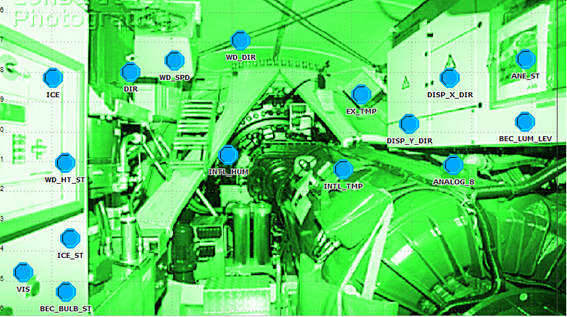
\includegraphics[width=\columnwidth]{Resim/Sekil4-2.png}}
\caption{Türbin içi \gls{wnac} modülünün temsili gösterimi (\protect\citeA{ltd_2005}).}
\label{fig:4-2}
\end{figure}


\begin{figure}[htbp]
\centerline{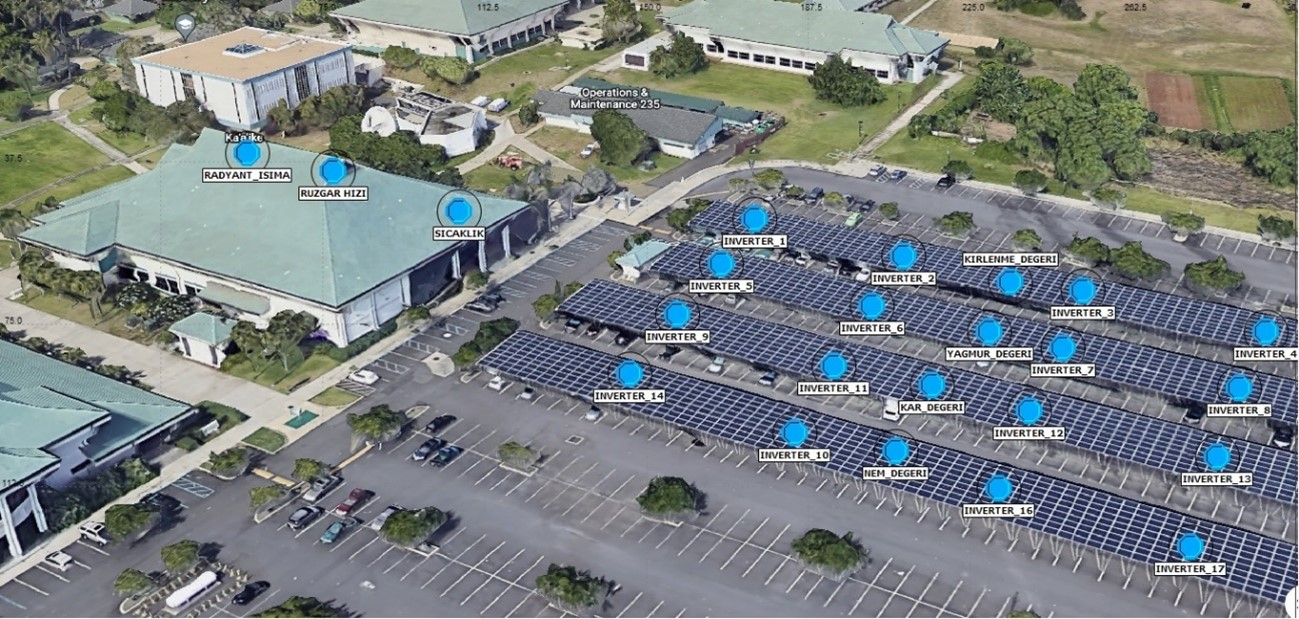
\includegraphics[width=\columnwidth]{Resim/sekil4-3.jpg}}
\caption{OPNET yazılımında güneş enerji sisteminde çalışan algılayıcı modüllerin gösterimi (\protect\citeA{inc_2015}).}
\label{fig:4-3}
\end{figure}


\subsection{Algılayıcı Düğümlerin Veri Boyutu Hesaplanması}\label{verboyut}

Bu bölüm, rüzgar türbini ve güneş enerji tarlalarında durum izleme ve arıza tahmini görevlerini gerçekleştirmek için çalışan algılayıcı düğümlerinin oluşturduğu veri boyutlarını açıklamaktadır. İlgili algılayıcıların temel prensipleri 4.1.1 ve 4.1.2 başlıkla-rında açıklanmıştır.


Yenilenebilir enerji sistemlerinde çalışan algılayıcı düğümlerinin oluşturdukları veri boyutu Denklem \eqref{eq4-1} ile bulunabilir \cite{ahmed2011simulation}.


\begin{equation}
\text{Veri hızı} = 2.\text{f\textsubscript{s}}(\text{Örnekleme frekansı}) \label{eq4-1}
\end{equation}

Mantıksal düğümlerden çıkan veriler örneklendiğinde 2 Byte’lık veri üretilecek şekilde tasarlanmıştır. Örnekleme frekansıyla çarpıldığı zaman mantıksal düğümün bir saniyede oluşturduğu veri boyutu hesaplanmış olur.

Mantıksal düğümler, ilgili bileşenle ilgili farklı türde bilgileri tutabilen bir verilerdir. Gerçek cihazla ilgili sanal model tarafından modellenen iyi bilinen fonksiyonlardır ve işlevselliğine dayalı bir veri listesi içerirler. Ek olarak mantıksal düğümlerde oluşan verilerin doğruluğu çok önemli olduğundan TCP/IP tekniği ile veri iletimi ve FTP uygulama katmanı ile çalışan bir haberleşme temelinde tasarlanmıştır. \cite{klise2017application} makalede tasarlanan veri modeli üzerinden gidildiğinde rüzgar enerji sistemi ve güneş enerji sisteminde çalışan algılayıcıların oluşturduğu veri boyutları Tablo \ref{tab:tablo4-4} ve Tablo \ref{tab:tablo4-5}’te gösterilmiştir.

\begin{table}[htbp]
\centering
\caption{Rüzgar türbinindeki algılayıcı gruplarının ürettiği veri boyutları}
\label{tab:tablo4-4}
\begin{tabular}{cccc}
\multicolumn{1}{c}{\begin{tabular}[c]{@{}c@{}}Algılayıcı modül\\ isimleri\end{tabular}} &
  \begin{tabular}[c]{@{}c@{}}Durum algılayıcı\\ veri boyutu (f\textsubscript{s} = 1)\end{tabular} &
  \begin{tabular}[c]{@{}c@{}}Analog algılayıcı\\ veri boyutu (f\textsubscript{s} = 500)\end{tabular} &
  \begin{tabular}[c]{@{}c@{}}Toplam aktarılan\\ veri\end{tabular} \\ \hline
WROT & 5*2*f\textsubscript{s} = 10 Byte/s & 12*2*f\textsubscript{s} = 12000 Byte/s     & 12010 Byte/s \\
WTRM & 8*2*f\textsubscript{s} = 16 Byte/s & 12*2*f\textsubscript{s} = 12000 Byte/s  & 12016 Byte/s \\
WGEN & 2*2*f\textsubscript{s} = 4 Byte/s  & 14*2*f\textsubscript{s} = 14000 Byte/s & 14004 Byte/s \\
WCNV & 2*2*f\textsubscript{s} = 4 Byte/s  & 15*2*f\textsubscript{s} = 15000 Byte/s & 15004 Byte/s \\
WTRF & 3*2*f\textsubscript{s} = 6 Byte/s  & 8*2*f\textsubscript{s} = 8000 Byte/s   & 8006 Byte/s  \\
\gls{wnac} & 4*2*f\textsubscript{s} = 8 Byte/s  & 11*2*f\textsubscript{s} = 11000 Byte/s & 11008 Byte/s \\
WYAW & 2*2*f\textsubscript{s} = 4 Byte/s  & 6*2*f\textsubscript{s} = 6000 Byte/s   & 6004 Byte/s  \\
WTOW & 3*2*f\textsubscript{s} = 6 Byte/s  & 2*2*f\textsubscript{s} = 2000 Byte/s   & 2006 Byte/s  \\
WMET & 0                  & 8*2*f\textsubscript{s}= 8000 Byte/s    & 8000 Byte/s 
\end{tabular}
\end{table}

Tablo \ref{tab:tablo4-4}'e göre rüzgar türbinindeki algılayıcı düğümlerinin yapısı için OPNET yazılımında “Application config” modülü eklenerek \gls{iec} 61400-25 ve \gls{iec} 61724 standartlarına göre ANALOG ve STATUS verileri Şekil \ref{fig:4-4}'teki gibi oluşturulur.“Application config” modülünde tasarlanan uygulama verilerinin, ağ senaryolarında kullanılması için “Profil Definition” modülüne entegre edilmesi gerekir. 

\begin{table}[htbp]
\centering
\caption{Güneş enerji tarlasındaki algılayıcı gruplarının ürettiği veri boyutları}
\label{tab:tablo4-5}
\begin{tabular}{lc}
\multicolumn{1}{c}{\begin{tabular}[c]{@{}c@{}}Algılayıcı modül isimleri\end{tabular}} & A sınıfı (yüksek tutarlılık periyodu) \\ \hline
Radyant ışıma              & 1*2*100 = 200 Byte/s    \\
Meteoroloji modülü               & 5*2*1 = 10 Byte/s       \\
Rüzgar hızı                & 1*2*3 = 6 Byte/s        \\
İnverter (Gerilim ve Akım) & 2*2*1440 = 28800 Byte/s
\end{tabular}
\end{table}

\begin{figure}[htbp]
\centerline{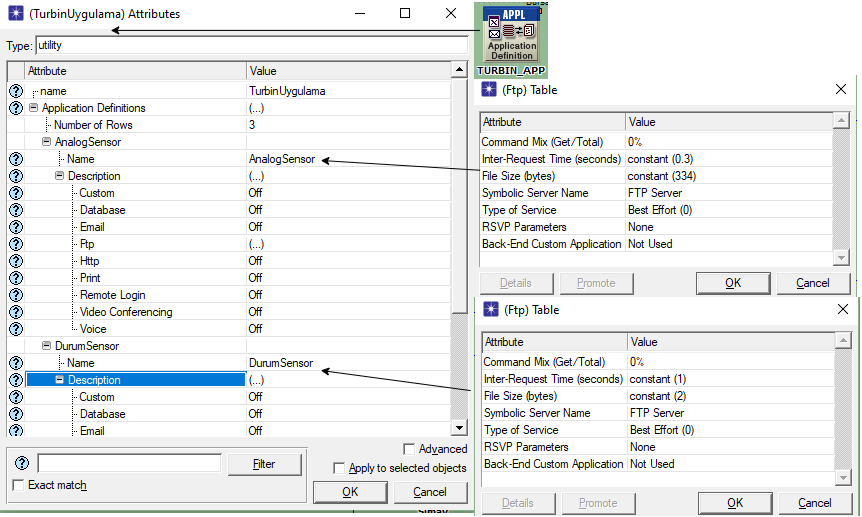
\includegraphics[width=\columnwidth]{Resim/sekil4-4.png}}
\caption{OPNET Yazılımında “Application Config” bölümü}
\label{fig:4-4}
\end{figure}

Örneğin, invertör profiline ait güneş panelinde voltaj ve akım algılayıcısı olarak iki adet algılayıcı modeli bulunmaktadır. Bu kritere göre OPNET yazılımının “Application Config” modülünde gerilim ve akım algılayıcılarının veri yapıları oluşturulur. İkinci aşamada ise oluşturulan bu veri yapıları “Profil Definition” modülü kullanılarak invertör profili çatısında toplanır. Böylelikle invertör, OPNET’in ağ senaryolarında kullanımı sağlanmış olur. Şekil \ref{fig:4-5}’te \gls{wnac} profilinin \gls{opnet} yazılım yapısı görülmektedir. Tablo \ref{tab:tablo4-4}’e göre \gls{wnac}'a ait olan algılayıcılar \gls{opnet} yazılımında kurulmuştur. Rüzgar türbininde enerji üretimi gerçekleşirken eş zamanlı çalışan \gls{wnac} gibi toplamda 9 adet algılayıcı düğüm modül grubu, güneş enerji sisteminde kullanılan 4 adet algılayıcı düğüm modül grubu, “Application config” ve “Profile config” bileşenleri kullanılarak simülasyon ortamında çalışan algılayıcı gruplarına dönüştürülmüştür.
\begin{figure}[htbp]
\centerline{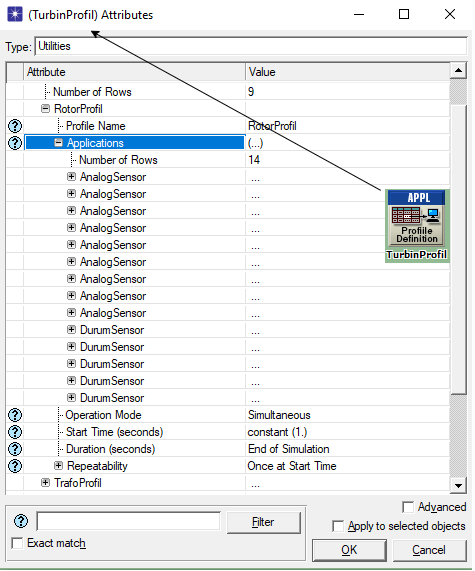
\includegraphics[width=5cm]{Resim/sekil4-5.png}}
\caption{OPNET Yazılımında “Profile Definition" bölümü}
\label{fig:4-5}
\end{figure}